\section{A spectral explanation in frozen features}
\label{sec:theory}\label{sec:rfnn}

The frozen-feature score model of \cref{sec:setup}, \eqref{eq:rfnn}, trained by gradient flow at a fixed diffusion time, is a setting in which the phenomenon of \cref{sec:phenomenon} can be solved rather than measured: each mode has an inverse-eigenvalue timescale governed by the feature correlation matrix $\Umat$ of \eqref{eq:U}, and the delay of memorization is a statement about the \emph{ratio} of two of its spectral edges. Full statements, hypotheses and proofs are in \cref{app:theory}; the model makes no claim about the trained networks of \cref{sec:phenomenon,sec:real}, which \cref{sec:real} tests separately.

\paragraph{Parallel mode dynamics.}\label{sec:theory-setup}
By \eqref{eq:rfnn-gradflow}, the readout coefficient along the $i$-th eigenvector of $\Umat$ relaxes to its target as $1-e^{-\lambda_iT}$, independently of every other direction (\cref{lem:gf-p1}). Each eigenvalue is a learning rate for one direction, and sorting the spectrum sorts the order of absorption. Writing $\mathcal S$ for the $\dint$ signal modes and $\mathcal M$ for the $\nsamp-\dlat$ sample-specific modes (\cref{prop:fourblock-9} below), define characteristic edge-absorption times at a common relative parameter tolerance $\varepsilon$ by
\begin{align}
\taugen&:=\log(1/\varepsilon)\big/\lambda^{\mathcal S}_{\min},\label{def:taugen-main}\\
\taumem^{\rm on}&:=\log(1/\varepsilon)\big/\lambda^{\mathcal M}_{\max}.\label{def:taumem-main}
\end{align}
These are spectral proxies: $\taugen$ tracks the slowest signal mode and $\taumem^{\rm on}$ the fastest index-defined sample-block mode. That block can contain population-aligned spikes, so its edge need not mark observed memorization onset. Relating it to the train--test gap requires the alignment assumptions and spike/bulk distinction of \cref{prop:gap-p1,def:taumem-p1}. Their ratio is independent of the common tolerance and clock normalization.

\paragraph{Four blocks and their edges.}\label{sec:theory-fourbulk}
Let $M_t=\tfrac1\nsamp\sum_\mu\E[x^\mu_tx^{\mu\top}_t]$ be the second moment of the noised training set, with population signal and null eigenvalues $\alpha_t^2=e^{-2t}(s^2/\dint+\sigsig^2)+\Delta_t$ and $\beta_t^2=e^{-2t}\signoise^2+\Delta_t$, and define the operating point
\begin{equation}\label{eq:fourbulk-q-main}
q(\dlat)=\frac{\operatorname{tr}M_t}{\dlat}=\beta_t^2+\frac{\dint(\alpha_t^2-\beta_t^2)}{\dlat},
\end{equation}
the input variance per coordinate seen by $\tanh$ (\cref{lem:q-p1}). Gaussian equivalence replaces $\tanh(\sqrt q z)$ by its linear part plus an independent residual, with coefficients $a_1(q)=\E[\tanh'(\sqrt qz)]$ and $a_*(q)^2=\E[\tanh(\sqrt qz)^2]-a_1(q)^2q$; both are evaluated at $q(\dlat)$, so nothing below is $\dlat$-independent.

\begin{proposition}[Four spectral blocks; sketched under Gaussian equivalence]\label{prop:fourblock-9}\label{prop:fourbulk-main}
Assume $\dint\ll\dlat<\nsamp<\pwidth$ with $\dint$ and $t>0$ fixed and $\dlat,\nsamp,\pwidth\to\infty$ at fixed $\gamma_\perp=(\dlat-\dint)/\nsamp$ and $\nsamp/\pwidth$; Gaussian equivalence of the feature Gram (\cref{ass:fourbulk-ge}); and $\signoise$ above the block-separation threshold $\signoise^*$ of \cref{prop:scope-sigperp} ($0.40$--$0.50$ for $\dlat\ge40$, satisfied at $\signoise=0.5$ and violated at $\signoise=0.01$). Then the sorted spectrum of $\Umat$ consists of four index blocks:
\begin{itemize}\setlength\itemsep{0pt}
\item[(i)] $\dint$ \emph{signal} outliers, population mean $a_1(q)^2\alpha_t^2/\dlat$, lifted by the null block as spiked-covariance perturbation theory prescribes \citep{baik2005phase};
\item[(ii)] $\dlat-\dint$ \emph{noise-dimension} modes of mean exactly $a_1(q)^2\beta_t^2/\dlat$, filling a Marchenko--Pastur band \citep{marchenko1967distribution} of support $\tfrac{a_1(q)^2}{\dlat}\bigl[e^{-2t}\signoise^2(1\pm\sqrt{\gamma_\perp})^2+\Delta_t\bigr]$;
\item[(iii)] $\nsamp-\dlat$ \emph{sample-specific} modes carrying the residual, nonlinear part of the features, mean $\simeq a_*(q)^2/\nsamp$ and top edge $\kappa_{\rm top}\,a_*(q)^2/\nsamp$;
\item[(iv)] $\pwidth-\nsamp$ \emph{residual-floor} modes, exact zeros for a single diffused copy.
\end{itemize}
Every data-side edge scales as $a_1(q(\dlat))^2/\dlat$ and is $\pwidth$-independent at leading order in $\dlat/\pwidth$; the sample block scales as $a_*(q(\dlat))^2/\nsamp$. The block means obey the exact trace identity
\begin{equation}\label{eq:fourbulk-trace-main}
\dint\frac{a_1^2\alpha_t^2}{\dlat}+(\dlat-\dint)\frac{a_1^2\beta_t^2}{\dlat}+\nsamp\frac{a_*^2}{\nsamp}=a_1(q)^2q+a_*(q)^2=\E\bigl[\tanh(\sqrt qz)^2\bigr],
\end{equation}
whose right side is $O(1)$ for every $\dlat$.
\end{proposition}
The counts follow from rank alone, by interlacing of a rank-$\dlat$ data term with the residual kernel (\cref{lem:fourbulk-counts,lem:fourbulk-bbp}, proved); the positions are sketched, and their drift with $\dlat$ through $q$ alone is reproduced with no fitted parameter in \cref{tab:fourbulk-numbers}, whereas a fixed-$a_1$ theory predicts flat blocks and is rejected. Blocks (i)--(ii) are disjoint iff $\lambda_{\min}(\hat C+\hat S_\parallel)>\signoise^2(1+\sqrt{\gamma_\perp})^2$, a condition in which $a_1^2$, $1/\dlat$ and $\pwidth$ cancel, and (ii)--(iii) are disjoint iff $\tfrac{\nsamp}{\dlat}\tfrac{a_1(q)^2}{a_*(q)^2}[e^{-2t}\signoise^2(1-\sqrt{\gamma_\perp})^2+\Delta_t]>\kappa_{\rm top}$ (\cref{app:theory-fourbulk}).\label{cor:fourbulk-separation-main} The measured spectra (\cref{fig:app-rfnn-exp2-pndr}) show the four blocks in every configuration, with the noise-dimension/sample gap at $0.6$--$1.3$ decades for $\signoise=0.5$ and closed at $\signoise=0.01$.

Theorem~3.1 of \citet{bonnaire2025} gives the limiting density of $\Umat$ for an arbitrary population spectral measure; \cref{prop:fourblock-9} is that theorem evaluated, not extended, at the two-atom measure $\tfrac{\dint}{\dlat}\delta_{\alpha_t^2}+(1-\tfrac{\dint}{\dlat})\delta_{\beta_t^2}$, blocks (i)--(ii) being their $\rho_2$ and block (iii) their $\rho_1$. \citet{george2025dsm} analyse a linear pencil with block dimensions $(\pwidth,\dlat-\dint,\dint,\nsamp)$ for data supported exactly on a $\dint$-dimensional subspace, the $\signoise=0$ limit in which (ii) and (iii) merge. What is new is strictly positive $\signoise$, which lifts (ii) off the sample bulk by $e^{-2t}\signoise^2$ with a Marchenko--Pastur width of ratio $\gamma_\perp$, and the reading of the blocks as gradient-flow learning-rate bands.

\paragraph{Spectral separation as a ratio of two edges.}\label{sec:theory-buffer}\label{prop:buffer-main}
Dividing the two absorption times, and inserting the edges of \cref{prop:fourblock-9} with $\ell_{\min}$ the smallest signal-subspace eigenvalue of the realised training set (\cref{prop:taugen-buf,prop:onset-buf}),
\begin{equation}\label{eq:R-main}
R(\dlat):=\frac{\taumem^{\rm on}}{\taugen}=\frac{\lambda^{\mathcal S}_{\min}}{\lambda^{\mathcal M}_{\max}}
=\frac{\nsamp}{\dlat}\cdot\frac{a_1(q)^2}{a_*(q)^2}\cdot\frac{e^{-2t}\ell_{\min}+\Delta_t}{\kappa_{\rm top}}\,\bigl(1+o(1)\bigr),
\end{equation}
with $q=q(\dlat)$ (\cref{cor:buffer-buf}).\label{cor:buffer-main} $R$ is \emph{not} a count of modes: the $\dlat-\dint$ noise-dimension modes multiply no absorption time, because a bound of the form (number of buffer modes)$\times$(time per mode) presumes that the flow traverses them sequentially, whereas under \eqref{eq:rfnn-gradflow} they decay in parallel with the rest of the spectrum and enter $R$ only through $q(\dlat)$, $\kappa_{\rm top}$ and $\ell_{\min}$ (\cref{rem:nonsequitur-buf}). $\dlat$ enters through the fan-in $1/\dlat$ of the data-side edges and through $q(\dlat)$, while $\ell_{\min}$ and $\kappa_{\rm top}$ also enter; growth of $a_1^2/a_*^2$ alone is not sufficient to guarantee increasing $R$. On the released spectra $\taugen$ grows $11\times$ in flow units over $\dlat=5\to200$ (it \emph{falls} in repository steps, $158\to43$), $\taumem^{\rm on}$ grows $221\times$, and $R$ grows monotonically from $21$ to $428$; predicted-versus-measured edges at every $\dlat$ are in \cref{app:theory}.

\paragraph{The operating point, and a fixed-$q$ control.}
What moves the edges is the de-saturation of $\tanh$. Over the sweep $q$ falls from $2.76$ to $0.33$, so $a_1^2$ rises from $0.18$ to $0.63$ and $a_*^2$ falls $17\times$ ($0.079\to0.0047$): the ratio $a_1^2/a_*^2$ grows $58\times$ and the sample-block top $\kappa_{\rm top}$ collapses $13\times$, while $\nsamp/\dlat$ shrinks $40\times$. Holding $q$ fixed removes the variation in the Hermite coefficients; the remaining dimension dependence tests their contribution to the growth of $R$. We hold the input variance per coordinate $q_{\rm in}=\E\|x\|^2/\dlat$ fixed by scaling $\signoise$ with $\dlat$ ($\signoise^2=(0.57\dlat-14)/(\dlat-\dint)$, coinciding with the $\signoise=0.5$ sweep at $\dlat=40$), and re-measure the spectrum at $\nsamp=500$, $\pwidth=4096$, $t=0.01$ over three seeds (\cref{rem:normfixed-buf}; \cref{fig:theory-main}). The intervention largely removes the endpoint growth, although the fixed-$q$ curve is non-monotone: $R$ changes $1.09\times$ over $\dlat=40\to240$ ($92,140,158,136,119,100$) against $3.17\times$ in the baseline ($92,145,201,266,287,291$), while the noise-dimension count grows $6.7\times$. The decomposition is the one \eqref{eq:R-main} predicts: $\lambda^{\mathcal S}_{\min}$ falls $4.3$--$4.4\times$ in both sweeps (the $1/\dlat$ of the signal edge), whereas the sample top falls $13.6\times$ in the baseline and only $4.8\times$ at fixed $q$, the missing factor being the shrinkage of $a_*(q)^2$. The isotropic control $\signoise=\sigsig$, where de-saturation is essentially absent, gives a non-monotone $R$ that peaks near $\dlat\approx40$ and then declines like $\nsamp/\dlat$ (\cref{rem:isotropic-buf}).

\begin{figure}[t]
  \centering
  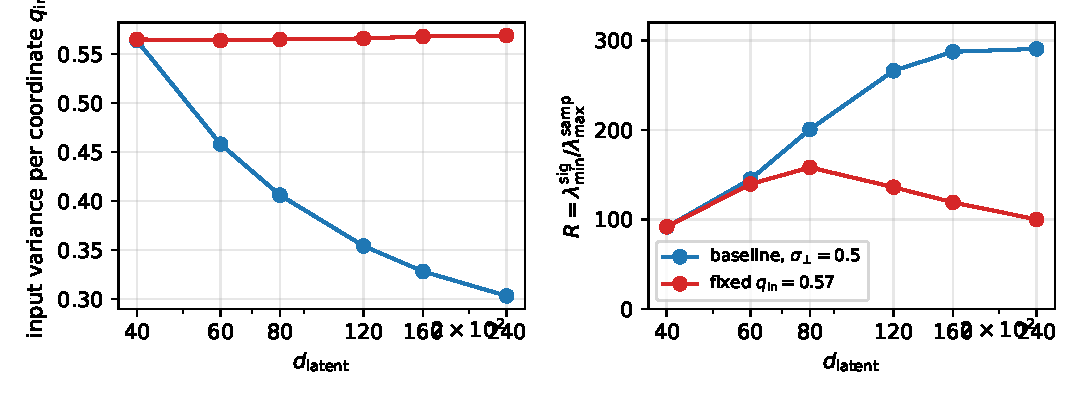
\includegraphics[width=0.92\linewidth]{figures/rfnn_fixed_q_control.pdf}
  \caption{\textbf{Fixed-$q$ control.} Left: the per-coordinate input variance $q_{\rm in}=\E\|x\|^2/\dlat$ along the $\signoise=0.5$ sweep (blue) and along a sweep in which $\signoise$ is scaled with $\dlat$ to hold $q_{\rm in}$ at its $\dlat=40$ value (red). Right: the edge ratio $R=\lambda^{\rm sig}_{\min}/\lambda^{\rm samp}_{\max}$ of the RFNN feature-correlation matrix ($\nsamp=500$, $\pwidth=4096$, $t=0.01$, three seeds). Holding the operating point fixed largely removes the endpoint growth of $R$ ($1.09\times$ against $3.17\times$ over $\dlat=40\to240$) while the noise-dimension count grows $6.7\times$. Representative spectra with the four blocks are in \cref{fig:app-rfnn-exp2-pndr}.}
  \label{fig:theory-main}
\end{figure}

\paragraph{What the model says.}\label{sec:theory-linear}\label{sec:theory-predictor}
Inside the frozen-feature model, lowering the operating point $q$ contributes to separating signal and sample-block absorption times, as supported by the fixed-$q$ control; the exactly solvable linear score model, the bridge from residual error to near-duplicate generation and the regime boundaries are in \cref{app:theory}. It says nothing about trainable first layers or adaptive optimizers, and whether any of it transfers to the trained networks is the question \cref{sec:real} puts to the data.
